\section{Introduction to Control Rods}

\subsection{Functions}
Control rods are essential for \textbf{modulating reactivity}, serving the following functions:
\begin{itemize}
    \item Compensating for excess reactivity due to fuel consumption or thermal feedback
    \item Regulating the neutron population
    \item Providing a safety margin for shutdown
    \item Assisting in reactor startup
\end{itemize}

\subsection{Physical Behavior}
Control rods function as \textbf{neutron absorbers} by altering the absorption component of $K_{eff}$:
\begin{equation}
    K_{eff} = \frac{Production}{Absorption + Leakages} = \frac{\int \int \nu \Sigma_f \phi dV dE}{\int \int _{fuel} \Sigma_a \phi dV dE + \dot{L}}
\end{equation}

\subsection{Effects}
The insertion of a control rod modifies the neutron flux distribution as shown in figure \ref{fig:flux_depression_cr_insertion}. Its effectiveness depends on its absorption capability and the neutron flux in its vicinity.
\begin{figure}[H]
    \centering
    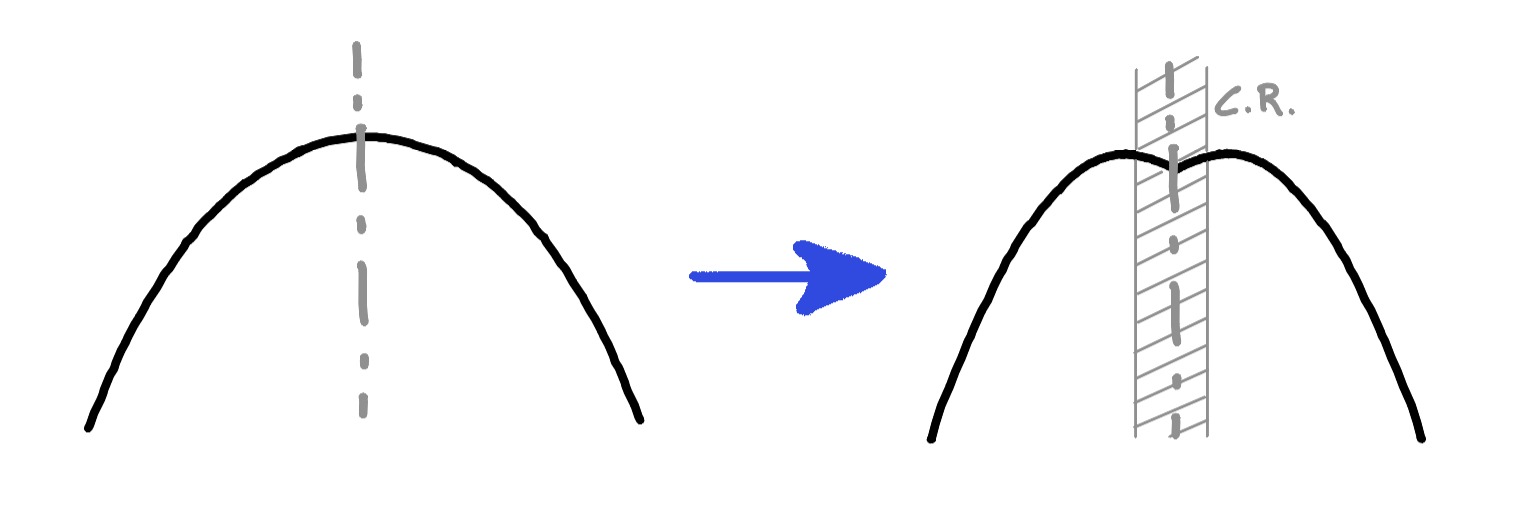
\includegraphics[width=0.75\linewidth]{CR_3.png}
    \caption{Flux before and after control rod insertion}
    \label{fig:flux_depression_cr_insertion}
\end{figure}

\textbf{Shadowing effect}: The position of one control rod can impact the effectiveness of another.

\subsection{Design}
The \textbf{material} selection is critical, requiring a substance with high absorption capabilities. For example, $B^{10}$ primarily undergoes (n,$\alpha$) reactions, while Gadolinium is more likely to produce (n,$\gamma$) reactions, which raises radiological safety concerns. \\
Following material selection, the \textbf{rod geometry} is typically constrained by overall design parameters. \\
Finally, the required \textbf{number of rods}, or equivalently the $pcm$, is determined by the need to compensate for excess reactivity at the start of the fuel cycle and provide an adequate shutdown margin. This depends on the core design and technology. 
For istance the difference between the excess reactivity over time in a conventional burner reactor agaist a breeeder reactor (shown in fig. \ref{fig:excess_reactivity_burner_vs_breeder}) shows the difference is needed reactivity compensation.

\begin{figure}[h]
    \centering
    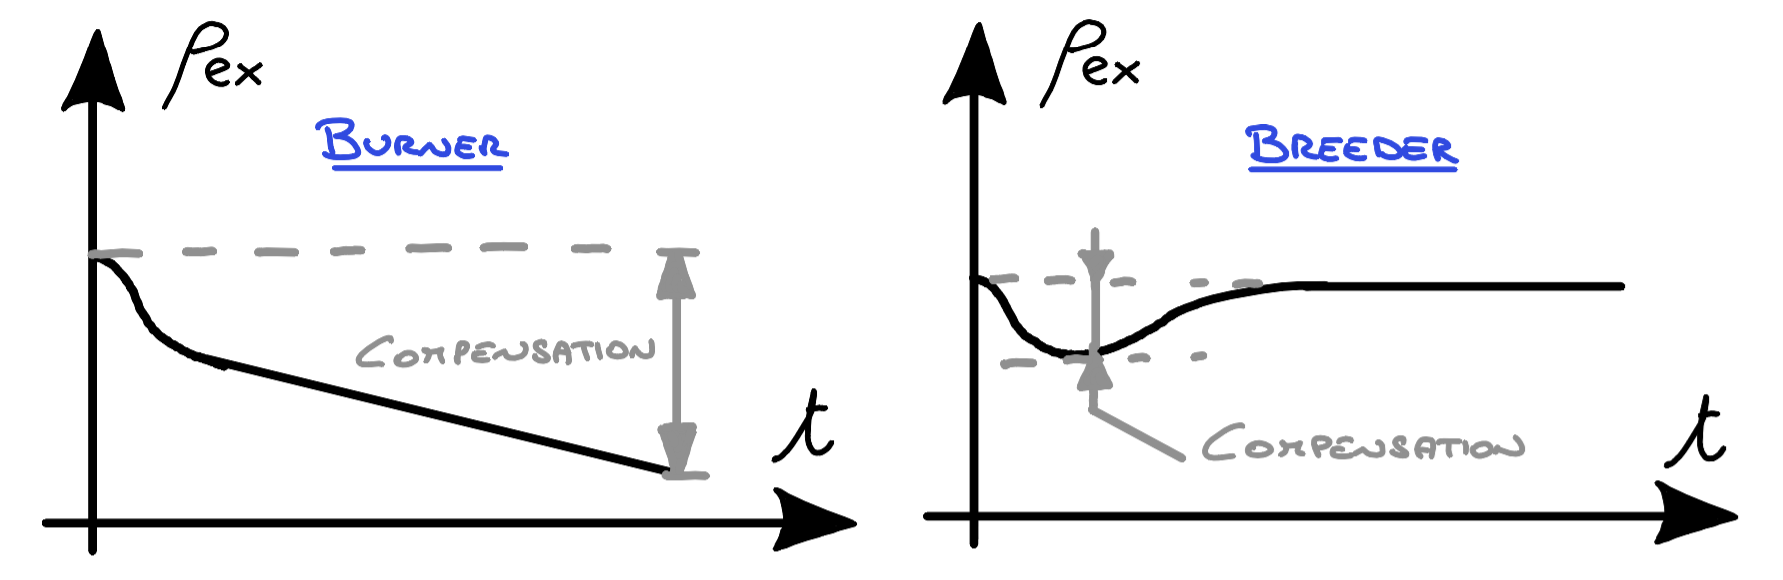
\includegraphics[width=0.75\linewidth]{CR_1.png}
    \caption{Reactivity worth needed for fuel consumption compensation is generally lower in breeder reactors compared to burner reactors.}
    \label{fig:excess_reactivity_burner_vs_breeder}
\end{figure}

\subsection{Calibration}
Calibration is necessary because the reactivity introduced by a control rod is not directly proportional to its insertion depth; instead, effectiveness varies with insertion depth, as illustrated in the following graphs:

\begin{figure}[h]
    \centering
    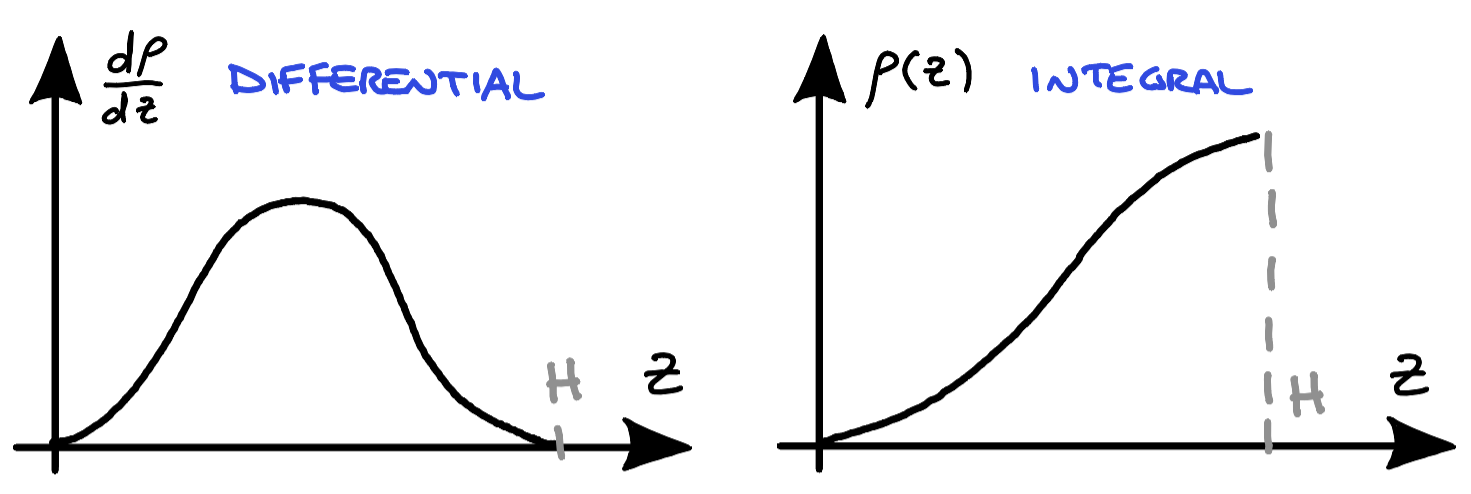
\includegraphics[width=0.75\linewidth]{CR_2.png}
    \caption{Differential and Integral reactivity curves}
\end{figure}


\subsection{Formulas}
The total reactivity worth ($\Delta \rho _{TOT}$) is given by:
\begin{equation}
    \Delta \rho _{TOT} = \Delta \rho _{SM} + \Delta \rho _{EX}
\end{equation}
where $\Delta \rho _{SM}$ is the shutdown margin and $\Delta \rho _{EX}$ is the reactivity excess.

Shutdown Margin:
\begin{equation}
    \Delta \rho _{SM} = \rho_i (\text{Criticality}) - \rho_i (\text{Fully IN}) 
\end{equation}
Reactivity excess:
\begin{equation}
    \Delta \rho _{EX} = \rho_i (\text{Fully OUT}) - \rho_i (\text{Criticality})
\end{equation}
